\chapter{Data and Representation}
\label{ch:3}
\noindent

\section{Datasets}
\subsection{Public Databases}
MassBank, pubChem, NIST
\subsection{Custom Dataset Construction}

\section{Preprocessing - Generating the Synthetic Data}
mod Derivation Graph
reason, goal: gives info of parents of fragments

\subsection{mod Strategy}
\paragraph{Forward strategy} builds a pipeline that 
\begin{enumerate}
    \item seeds the derivation graph with the molecule via \texttt{mod.addSubset}, 
    \item applies exactly one ionization step wrapped in \texttt{sub\_group} to constrain it to the current derivation graph, and then 
    \item  applies up to \texttt{frag\_repeat} fragmentation steps, 
    \item but only keeps paths whose intermediate fragments satisfy both mass bounds and charge bounds via nested \texttt{amu\_bound} and \texttt{charge\_bound} filters.
\end{enumerate}

\paragraph{Backward strategy} 
\begin{enumerate}
    \item seeds the derivation graph with the provided fragment graphs via \texttt{mod.addSubset}, 
    \item then applies up to \texttt{frag\_repeat} fragmentation rules scoped to the derivation graph, 
    \item while filtering intermediates to keep only fragments within the given mass window and valid charge bounds (nested \texttt{amu\_bound} inside \texttt{charge\_bound}).
\end{enumerate}


\subsection{computation times}

an improve is needed to make this aproach feasable
also this is only a part of the rules that are known
the compute time per molecule will rise even more


regression analasis, performed

assumption:
\begin{itemize}
    \item Linearity
    \item Homoscedasticity
    \item Independence of Errors
\end{itemize}


\begin{figure}
    \centering
    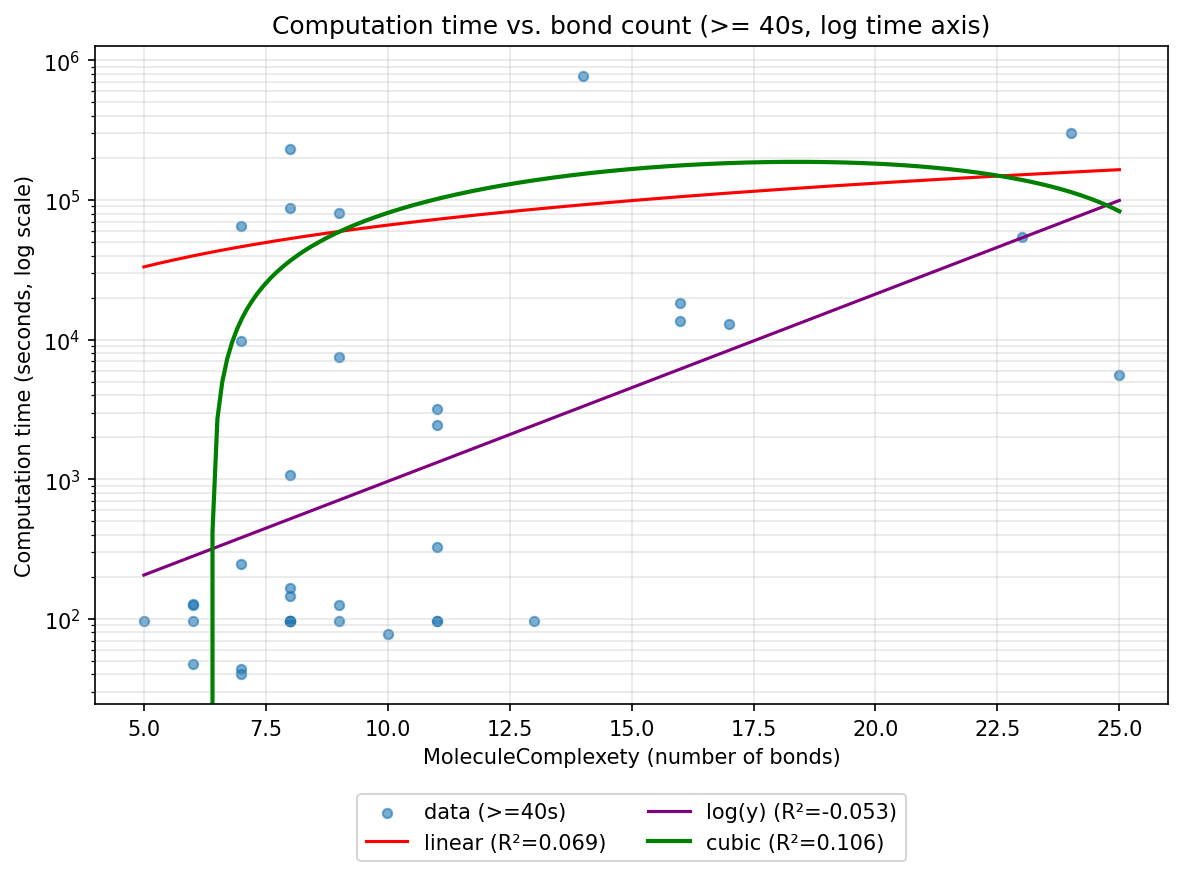
\includegraphics[width=0.75\linewidth]{time_vs_complexity_logy_over40.png}
    \caption{Regession of Computation time, filterd of molecules that took at least 40sec to compute}
    \label{fig:mod-time-regres}
\end{figure}

threshold of 40sec as the computation might not be very good


\section{Latend Representation Schemes}
\subsection{Molecular Graph Encoding}
py-geometric
\subsection{Fragment Graph Representation}
technically the same as the Molecular Graph
Vertex is a Atom
 with attributes like element type
Edge is a Bond
 with attributes 
 bond strengh
 half bond strength is aromaticity
\subsection{Spectral Vector and Embedding Representation}
latend represantation of the ms spectra
\subsection{Fragment–Spectrum Mapping}
How spectra and fragments are aligned.
The “fragment graph” concept - linking structure and spectral space.